\documentclass{beamer}

\mode<presentation>
{
  \usetheme{GTRI}
  %\useoutertheme{infolines}

  % or ...

 %\setbeamercovered{transparent}
  % or whatever (possibly just delete it)
}
\setbeamertemplate{navigation symbols}{}
\setbeamertemplate{footline}[page number]{}

\usepackage{fancybox}
\usepackage{listings}
\usepackage[abbr]{harvard}

\usepackage[english]{babel}
% or whatever

\usepackage[latin1]{inputenc}
% or whatever

\usepackage{times}
\usepackage[T1]{fontenc}
% Or whatever. Note that the encoding and the font should match. If T1
% does not look nice, try deleting the line with the fontenc.

\hypersetup{colorlinks=true,urlcolor=blue,linkcolor=black}


% "define" Scala
\lstdefinelanguage{scala}{
  morekeywords={abstract,case,catch,class,def,%
    do,else,extends,false,final,finally,%
    for,if,implicit,import,match,mixin,%
    new,null,object,override,package,%
    private,protected,requires,return,sealed,%
    super,this,throw,trait,true,try,%
    type,val,var,while,with,yield},
  otherkeywords={=>,<-,<\%,<:,>:,\#,@},
  sensitive=true,
  morecomment=[l]{//},
  morecomment=[n]{/*}{*/},
  morestring=[b]",
  morestring=[b]',
  morestring=[b]"""
}

\usepackage{color}
\definecolor{dkgreen}{rgb}{0,0.6,0}
\definecolor{gray}{rgb}{0.5,0.5,0.5}
\definecolor{mauve}{rgb}{0.58,0,0.82}
 
% Default settings for code listings
\lstset{frame=tb,
  %language=scala,
  aboveskip=3mm,
  belowskip=3mm,
  showstringspaces=false,
  columns=flexible,
  basicstyle={\scriptsize\ttfamily},
  numbers=none,
  numberstyle=\tiny\color{gray},
  keywordstyle=\color{blue},
  commentstyle=\color{dkgreen},
  stringstyle=\color{mauve},
  frame=single,
  breaklines=true,
  breakatwhitespace=true
  %tabsize=3
}


\title[Information Systems] % (optional, use only with long
                                      % paper titles)
{PMASE - Information Systems}

\subtitle{Lecture 02: Hardware}
%% {Include Only If Paper Has a Subtitle}

\author[Chris Simpkins] % (optional, use only with lots of authors)
{Christopher Simpkins\\\href{mailto:chris.simpkins@gtri.gatech.edu}{chris.simpkins@gtri.gatech.edu}\\\href{http://www.cc.gatech.edu/~simpkins/}{http://www.cc.gatech.edu/$\sim$simpkins/}}
% - Give the names in the same order as the appear in the paper.
% - Use the \inst{?} command only if the authors have different
%   affiliation.

\institute[GTRI] % (optional, but mostly needed)

\date[] % (optional, should be abbreviation of
                           % conference name)
{}
\subject{Information Systems Engineering}
% This is only inserted into the PDF information catalog. Can be left
% out. 


\begin{document}


\begin{frame}{ASE 6121 Information Systems}

\begin{center}
{\LARGE Lecture 02: Computers}\\
\vspace{.2in}
{\Large Christopher Simpkins}\\
{\large \href{mailto:chris.simpkins@gatech.edu}{chris.simpkins@gatech.edu}}\\
{\large \href{http://www.cc.gatech.edu/~simpkins/}{http://www.cc.gatech.edu/$\sim$simpkins/}}
\end{center}

\end{frame}

% --------------------------------------------------------------------------
\begin{frame}{Computers}

\begin{center}
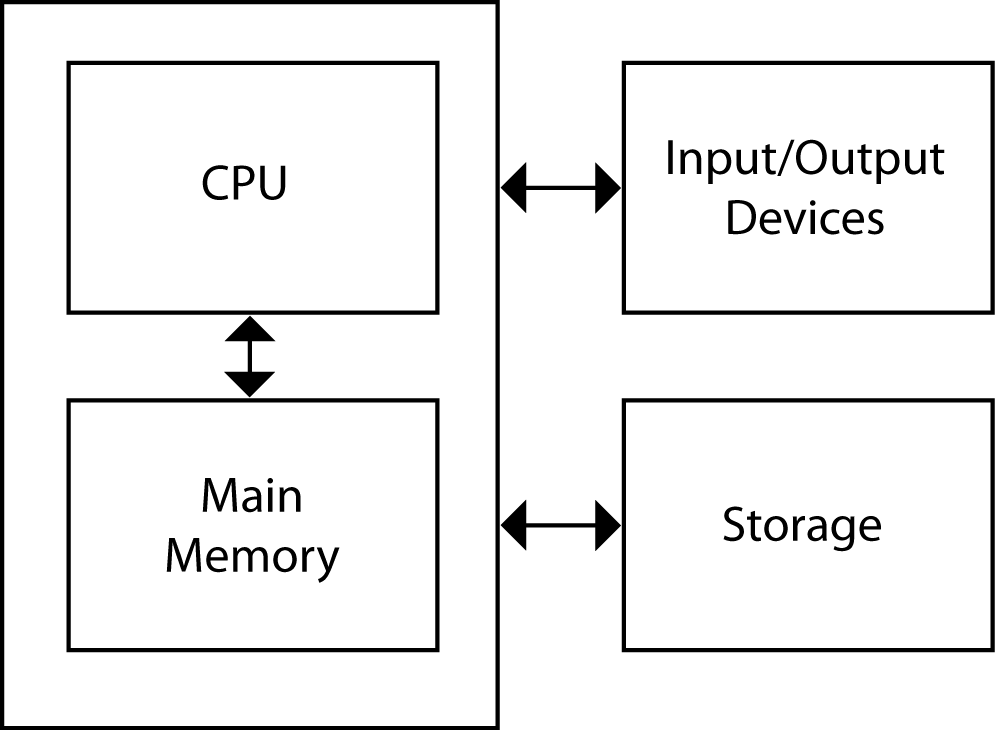
\includegraphics[height=2.5in]{computer-block-diagram.png}
\end{center}
Functional view of the major subsystems of a computer.  
\end{frame}
% --------------------------------------------------------------------------

% --------------------------------------------------------------------------
\begin{frame}{Computer Hardware}

\begin{center}
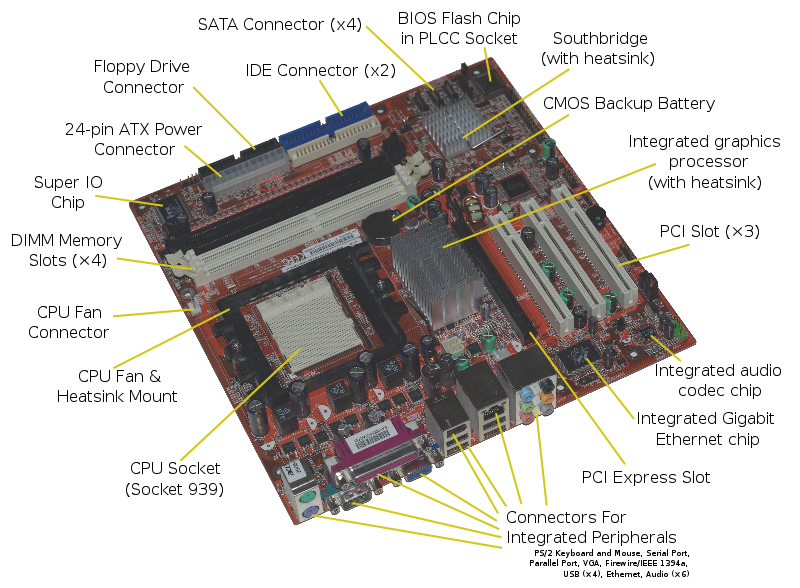
\includegraphics[height=2.4in]{acer-motherboard.png}\footnote{Source:
  \url{http://en.wikipedia.org/wiki/File:Acer_E360_Socket_939_motherboard_by_Foxconn.svg}}
\end{center}
A computer motherboard housing the CPU, main memory, I/O controllers,
and I/O ports.

\end{frame}
% --------------------------------------------------------------------------

% --------------------------------------------------------------------------
\begin{frame}{Central Processing Unit}

The ``brain'' of the computer.  In the von-Neumann architecture, the
CPU fetches an instruction from memory, executes the instruction,
possibly writes something to memory, then repeats the cycle.  Core
components of a microporocessor are arithmetic-logic unit (ALU) and
control unit.  CPU is implemented as a microprocessor
\begin{itemize}
\item RISC (Reduced Instruction Set Computing) processors have small,
  fast-executing instruction sets.  All modern microprocessors are
  RISC
\item CISC (Complex Instruction Set Computing) processors have large
  instruction sets and complicated addressing modes that slow all
  instructions down.  Notably, the Intel x86 architecture was
  originally CISC but is now RISC
\end{itemize}
\end{frame}
% --------------------------------------------------------------------------

% --------------------------------------------------------------------------
\begin{frame}{CPU Performance}

How to compare CPUs?
\begin{itemize}
\item Clock speed, typically measured in GHz, indicates the number of
  instructions that can be executed in a second
\item Modern pipelined processors are superscalar, meaning they can
  execute more than one instruction per clock cycle.
\item Benchmarks such as FLOPS (floating-point operations persecond)
  can help, but hard to isolate non-CPU factors such as memory speed,
  cache performance, etc.
\item Best benchmarks are suites of real-world application tests using
  wall-clock time - these tests compare computers, not necessarily
  isolating CPUs
\end{itemize}
\end{frame}
% --------------------------------------------------------------------------

% --------------------------------------------------------------------------
\begin{frame}{Multicore Processors}

\begin{columns}[t]
\begin{column}{2.8in}
\begin{center}
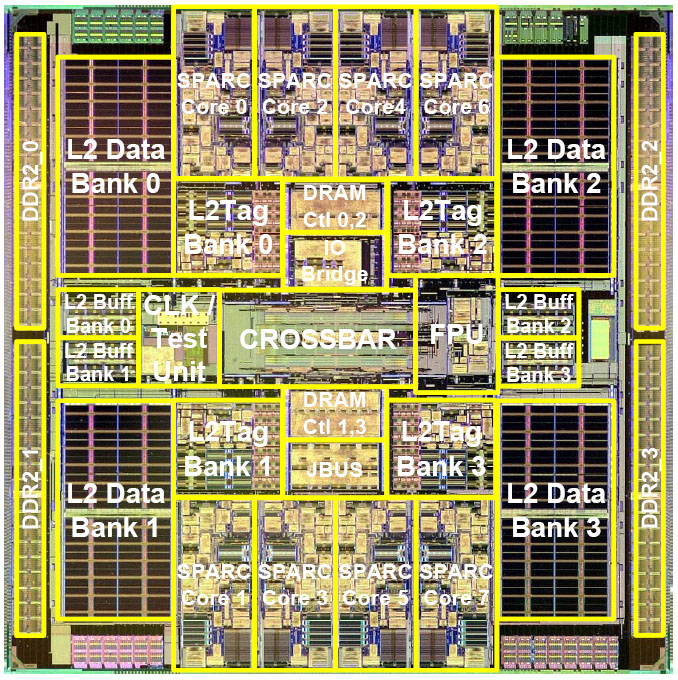
\includegraphics[width=2.5in]{ultrasparc-die.jpg}\footnote{Source: \url{http://jinsatoh.jp/ennui/ultrasparcT1_overlay_die.jpg}}
\end{center}
\end{column}
\begin{column}{2.2in}
\begin{itemize}
\item Trend is toward multi-core processors, which have multiple
  processing cores on a single chip.  Each core is like a CPU, with an
  ALU, control unit, registers, and optionally dedicated Level 1 cache
  memory
\item The Sun UltraSPARC T1 pictured here has 8 processing cores
\end{itemize}
\end{column}
\end{columns}

\end{frame}
% --------------------------------------------------------------------------

% --------------------------------------------------------------------------
\begin{frame}{32-Bit  and 64-Bit Processors}

What does it mean to have a 32-bit or 64-bit processor?
\begin{itemize}
\item Processor registers hold operands, intermediate computation
  results, and values that represent memory locations
\item Word size is the size of the processor registers.  A 32-bit
  processor has 32-bit registers (4 bytes - a byte is 8 bits)
\item Memory address busses are typically the same width as the word
  size, which makes memory access very fast
\item Wider memory busses mean more addressable memory.
\item 32-bit processors can typically address 4 GB of RAM
  ($2^{32}$)
\item 64-bit processors can typically address (in theory) $2^{64}$ =
  18 EB (exabytes - $18x10^{18}$ bytes) of RAM
\item Addressing more RAM means holding bigger data structures, like
  massive arrays, in memory
\end{itemize}
\footnote{Note that memory is byte-addressable, regardless
  of word size}
\end{frame}
% --------------------------------------------------------------------------

% --------------------------------------------------------------------------
\begin{frame}{Main Memory}

\begin{columns}
\begin{column}{2.5in}
\begin{center}
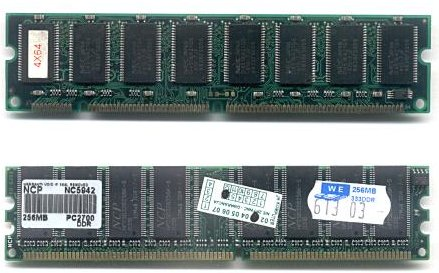
\includegraphics[width=2in]{dimms.jpg}

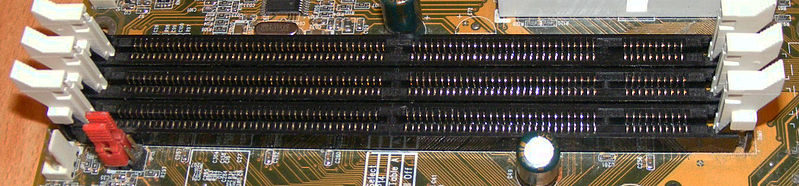
\includegraphics[width=2in]{dimm-sockets.jpg}
\end{center}
\end{column}
\begin{column}{2.5in}
\begin{itemize}
\item Random access memory (RAM)
\item Where running programs and data are stored
\item Typically housed in dual-inline memory modules (DIMMs) that
  insert easily into slots, pictured to the left
\end{itemize}
\end{column}
\end{columns}
\footnote{Source: \url{http://en.wikipedia.org/wiki/File:DIMMs.jpg}}
\footnote{Source: \url{http://en.wikipedia.org/wiki/File:3SDRAM-DIMMs.jpg}}
\end{frame}
% --------------------------------------------------------------------------

% --------------------------------------------------------------------------
\begin{frame}{Storage}


\begin{columns}[t]
\begin{column}{2.5in}
\begin{center}
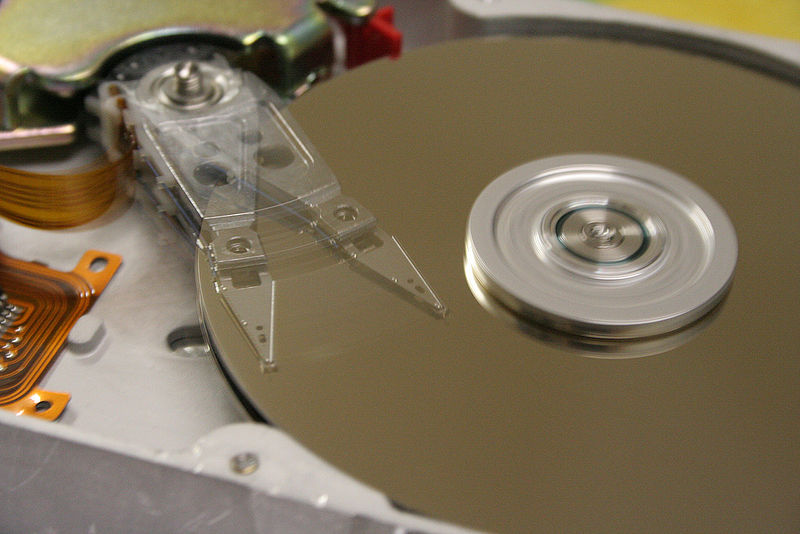
\includegraphics[width=2in]{hdd-spin.jpg}
\end{center}
\small A spinning hard disk with
the read-write heads moving over the platters.  Data stored in
magnetic particles on platters.  ``Head crashes'' are possible,
especially if HDD is jarred.
\normalsize
\end{column}
\begin{column}{2.5in}
Where programs and data are stored when not in use.
\begin{itemize}
\item Hard disk drives (HDDs) most common.  Good trade-off between cost and
  performance
\item Solid-state drives (SDDs) becoming more common.  Much faster
  than HDDs, more reliable (no moving parts), but much more expensive
\item Tapes and optical drive slow and sometimes write-only.  Used for
  long-term archiving
\end{itemize}
\end{column}
\end{columns}
\footnote{Source: \url{http://www.flickr.com/photos/alphasix/158829630/}}

\end{frame}
% --------------------------------------------------------------------------

% --------------------------------------------------------------------------
\begin{frame}{The Memory Hierarchy}

\vspace{-.15in}
\begin{columns}
\begin{column}{6in}
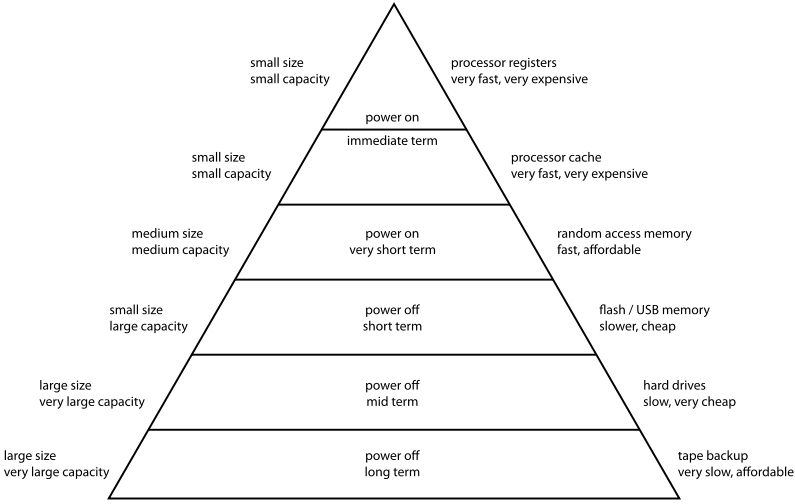
\includegraphics[height=3.1in]{memory-hierarchy.png}
\end{column}
\end{columns}
\scriptsize \url{http://en.wikipedia.org/wiki/File:ComputerMemoryHierarchy.svg} \normalsize
\end{frame}
% --------------------------------------------------------------------------

% --------------------------------------------------------------------------
\begin{frame}{Input/Output Devices}

Input devices convert physical phenomena into electrical signals that are
then converted to readable bits in the computer (see Sensors class
material for more):
\begin{itemize}
\item Keyboard
\item Camera
\item Microphone
\item Accelerometer
\item Gyroscope
\end{itemize}
Output devices convert bits from the computer into forms perceptible
to humans:
\begin{itemize}
\item Display monitor
\item Speakers
\end{itemize}
Note that input/output (I/O) also refers to communication with
anything external to the CPU and memory, for example, disk I/O or
network I/O
\end{frame}
% --------------------------------------------------------------------------

% --------------------------------------------------------------------------
\begin{frame}{Software}

\begin{columns}
\begin{column}{2.2in}
\begin{center}
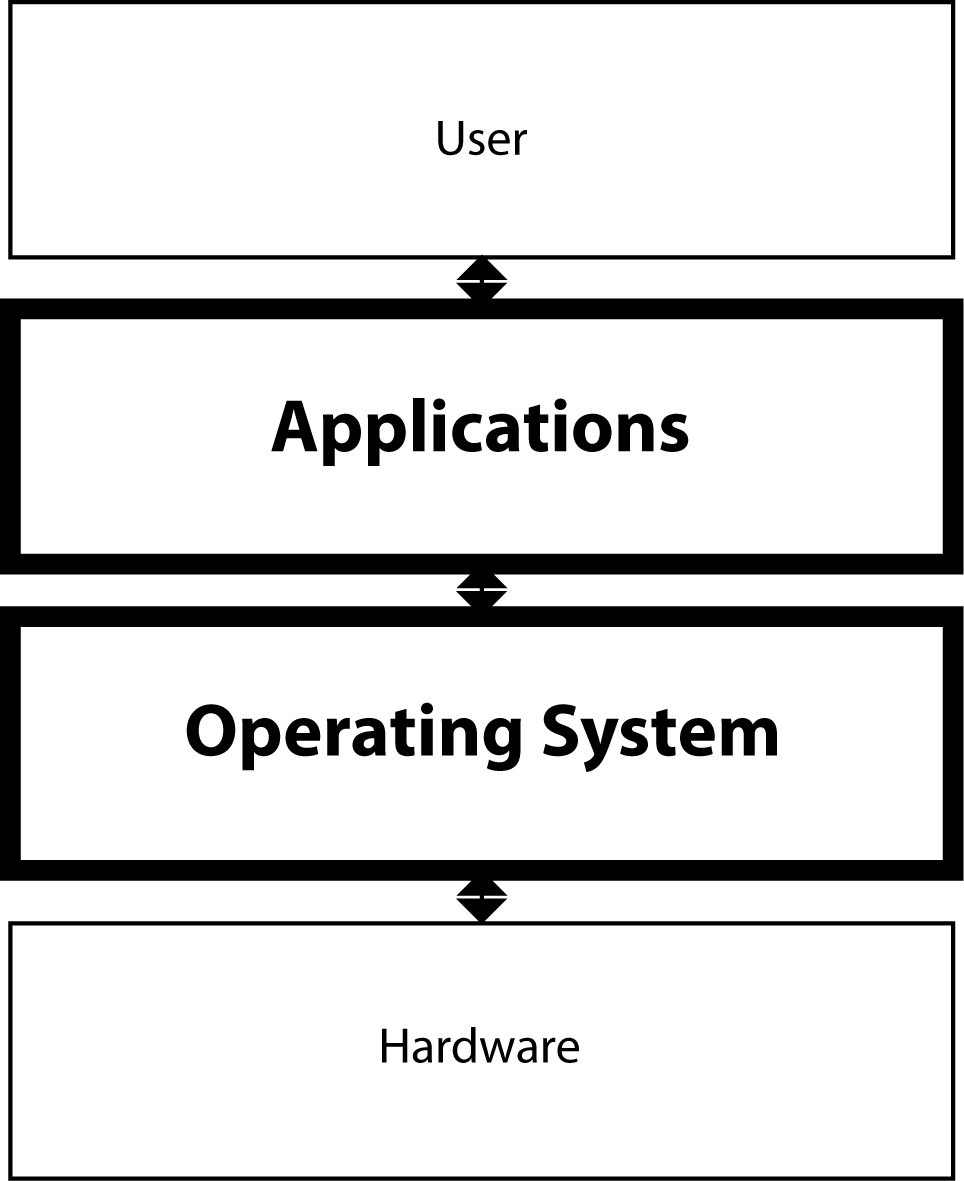
\includegraphics[width=2in]{applications-os.png}
\end{center}
\end{column}
\begin{column}{2.6in}
Two kinds of software:
\begin{itemize}
\item Application software: what the users interact with.  Web
  browsers, email clients, spreadsheets, text editors, etc.
\item System software: what the applications interact with.  File
  systems, device drivers, network services, etc.
\end{itemize}
Each layer of the computer system abstracts the layer below
\end{column}
\end{columns}

\end{frame}
% --------------------------------------------------------------------------

% --------------------------------------------------------------------------
\begin{frame}{Operating Systems}
Rough definition of operating system: the software that controls the
hardware.
Operating systems provide:
\begin{itemize}
\item a file system, so application programs can deal with files and
  directories instead of sectors and tracks;
\item process scheduling, so multiple programs can run concurrently
  and share resources such as the processor;
\item device drivers, so programs can interact with devices uniformly
  rather than having to know details of many different versions of
  devices; and
\item virtual memory management, so that programs can be given a
  simple, large enough memory space to run even when physical RAM is
  limited.
\end{itemize}

\end{frame}
% --------------------------------------------------------------------------

% --------------------------------------------------------------------------
\begin{frame}{Virtual Memory}

\begin{columns}
\begin{column}{2.2in}
\begin{center}
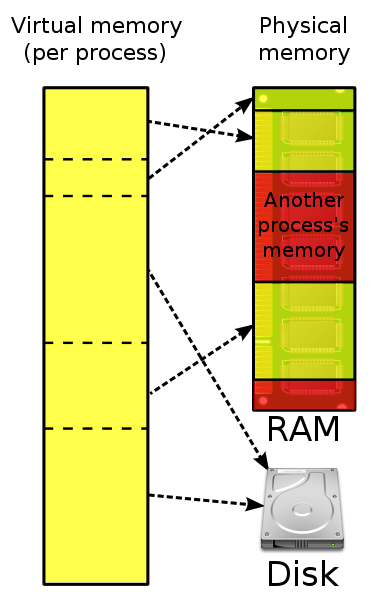
\includegraphics[width=1.8in]{virtual-memory.png}\footnote{\url{http://en.wikipedia.org/wiki/File:Virtual_memory.svg}}
\end{center}
\end{column}
\begin{column}{2.6in}
Programs and their data rarely fit in physical RAM
\begin{itemize}
\item OS swaps pages not currently used to disk, reloads them when
  needed
\item When a memory location that's on disk is accessed, the page that
  contains it is swapped back into physical RAM
\item This process gives rise to the ``clicking'' you hear from your
  disk drive when you launch a program
\item Disks are slow compared to RAM
\end{itemize}
Take-away lesson: if you're swapping a lot (lots of disk activity),
adding physical RAM will improve your computer's performance
\end{column}
\end{columns}
\end{frame}
% --------------------------------------------------------------------------

% --------------------------------------------------------------------------
\begin{frame}{Consequences of the Memory Hierarchy}

\begin{itemize}
\item Typical CPUs run at 2 GHz or more, RAM is typically 1 GHz,
  meaning that when the processor must access RAM, it waits for data
  for at least one instruction cycle
\item RAM can be accessed on the order of nanoseconds ($10^{-9}$)
\item Hard disks typically accessed on the order of milliseconds ($10^{-3}$)
\item When programs access the disk, or the operating system's virtual
  memory manager performs paging operations, performance suffers
\item Conclusion: large caches and lots of RAM mean higher performance
\end{itemize}

\end{frame}
% --------------------------------------------------------------------------

% --------------------------------------------------------------------------
\begin{frame}{Applications}

Now we're familiar with the hardware and software platform that
applications run on.
\begin{itemize}
\item Hardware houses all the software and constrains performance
  characterstics by processor speeds and memory architectures
\item Operating systems provide a unified view of the hardware and
  simplified execution environment for applications
\end{itemize}
Most of the remainder of this course will be primarily concerned with
application software

\end{frame}
% --------------------------------------------------------------------------

%% % --------------------------------------------------------------------------
%% \begin{frame}{}

%% \begin{itemize}
%% \item
%% \end{itemize}

%% \end{frame}
%% % --------------------------------------------------------------------------

%% % --------------------------------------------------------------------------
%% \begin{frame}{}

%% \begin{itemize}
%% \item
%% \end{itemize}

%% \end{frame}
%% % --------------------------------------------------------------------------



\end{document}
